% svg-padding: 4pt
\ifdefined\pdfoutput
  \ifnum\pdfoutput=0 \def\pgfsysdriver{pgfsys-dvisvgm.def}\fi
\fi
\documentclass[tikz,border=8pt]{standalone}
\usepackage{amsmath,amssymb}
\usetikzlibrary{arrows.meta}
\begin{document}
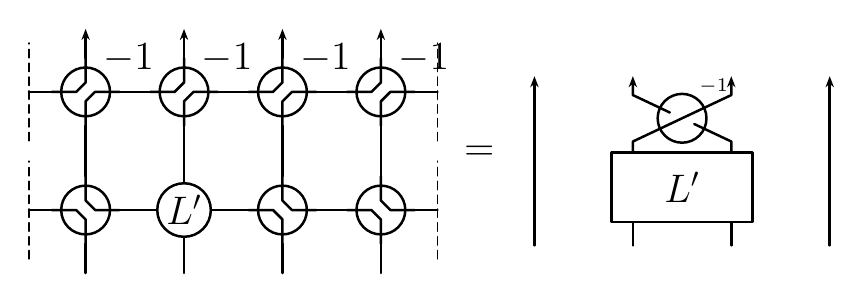
\begin{tikzpicture}[font=\Large,line width=.9pt,line cap=round,line join=round,>={Stealth[length=4pt]}]
% Four physical strands. Read operators from bottom (input) to top (output).
% An ordinary swap is TWO separate elbows, never a four-way junction.
% Circular boundaries denote local L(0) tensors, including their scalar.
% A superscript inverse on the boundary denotes the inverse local tensor.
\newcommand{\xxzTensorBoundary}[2]{\draw (#1,#2) circle (.31);}
\newcommand{\xxzSwap}[3]{%
 \xxzTensorBoundary{#1}{#2}
 \ifnum#3=0 \node[font=\Large,anchor=south west,inner sep=0pt] at (#1+.21,#2+.23) {$-1$};\fi
 \ifnum#3=1
  \draw (#1,#2-.43)--(#1,#2-.12)--(#1-.12,#2)--(#1-.43,#2);
  \draw (#1+.43,#2)--(#1+.12,#2)--(#1,#2+.12)--(#1,#2+.43);
 \else
  \draw (#1,#2-.43)--(#1,#2-.12)--(#1+.12,#2)--(#1+.43,#2);
  \draw (#1-.43,#2)--(#1-.12,#2)--(#1,#2+.12)--(#1,#2+.43);
 \fi}
\newcommand{\xxzDerivative}[2]{%
 \draw (#1,#2-.43)--(#1,#2+.43);
 \draw (#1-.43,#2)--(#1+.43,#2);
 \draw[fill=white] (#1,#2) circle (.34);
 \node at (#1,#2) {$L'$};}
\newcommand{\xxzRow}[3]{%
 % row y, orientation, derivative site (0 means no insertion)
 \foreach \j in {1,...,4}{%
  \pgfmathsetmacro{\xx}{1.25*(\j-1)}
  \ifnum\j=#3 \xxzDerivative{\xx}{#1}\else\xxzSwap{\xx}{#1}{#2}\fi}
 \foreach \j in {0,...,2}{\draw (1.25*\j+.43,#1)--(1.25*\j+.82,#1);}}
% Matching dashed cuts indicate the same periodic auxiliary space.
\newcommand{\xxzPeriodicEnds}[1]{%
 \draw (-.43,#1)--(-.72,#1);
 \draw (4.18,#1)--(4.47,#1);
 \draw[densely dashed,line width=.6pt] (-.72,#1-.62)--(-.72,#1+.62);
 \draw[densely dashed,line width=.6pt] (4.47,#1-.62)--(4.47,#1+.62);}
\newcommand{\xxzSiteLabels}[1]{%
 \foreach \j in {1,...,4}{\node at ({1.25*(\j-1)},#1) {$\j$};}}

\xxzRow{0}{1}{2}
\xxzRow{1.5}{0}{0}
\foreach \j in {0,...,3}{
 \draw (1.25*\j,.43)--(1.25*\j,1.07);
 \draw (1.25*\j,-.43)--(1.25*\j,-.8);
 \draw[->] (1.25*\j,1.93)--(1.25*\j,2.3);}
\xxzPeriodicEnds{0}
\xxzPeriodicEnds{1.5}
% Straightening the regular strands leaves P L' on inputs 2 and 3.
\node at (5.0,.72) {$=$};
\begin{scope}[xshift=5.7cm,yshift=.35cm]
 \foreach \j in {0,3}{\draw[->] (1.25*\j,-.8)--(1.25*\j,1.35);}
 % The lower tensor is L' on the two adjacent physical spaces.
 \draw (1.25,-.8)--(1.25,-.5);
 \draw (2.5,-.8)--(2.5,-.5);
 \draw[fill=white] (.98,-.5) rectangle (2.77,.38);
 \node at (1.875,-.06) {$L'$};
 % Inverse regular tensor above L': same four legs, with inverse weight.
 \xxzTensorBoundary{1.875}{.815}
 \node[font=\scriptsize,anchor=south west,inner sep=0pt] at (2.08,1.11) {$-1$};
 \draw[->] (1.25,.38)--(1.25,.52)--(2.5,1.11)--(2.5,1.35);
 \draw (2.5,.38)--(2.5,.52)--(2.03,.742);
 \draw[->] (1.72,.888)--(1.25,1.11)--(1.25,1.35);
\end{scope}
\end{tikzpicture}
\end{document}
